\section{Power Supply}
\subsection{Design Criteria}
\begin{outline}[enumerate]
\1 Size and weight: These could conflict however, if the size is no bigger than 4 cubic inches and all of the parts are surface mount, the heaviest part is the transformer. The power supply should not exceed 3 pounds if possible.
\1 Output voltage: The output voltage will need to be sufficient for various loads. It will need to still remain at 5V
\1  Efficiency: This is very important. Linear power supplies are not very efficient, which is why the team decided to build a switched-mode power supply. They are generally 30\% more efficient than linear power supplies. 
\1 Power Dissipation: Power dissipation shall be low.
\1 Electronic noise at input and outputs: The electronic noise at input and outputs shall not get to the point where compensation for noise is needed.
\end{outline}
\subsection{Alternatives}
\subsubsection{Buck converter}
 ``The input voltage is converted into a lower output voltage.''\cite{SMPSD}
\begin{figure}[h]
\begin{center}
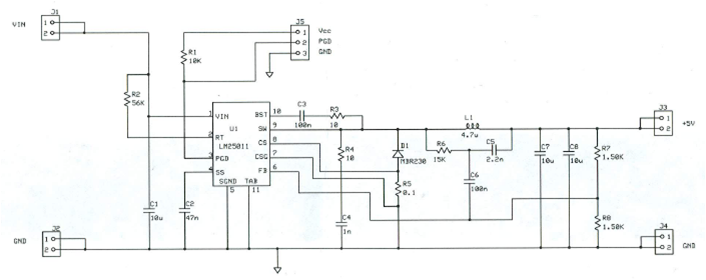
\includegraphics[width=4in]{includes/Buck}
\caption{Buck Converter}
\end{center}
\end{figure}


\subsubsection{A boost converter} 
``The input voltage is converted into a higher output voltage''\cite{SMPSD}
\begin{figure}[H]
\begin{center}
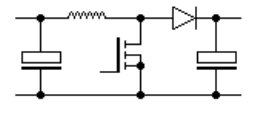
\includegraphics[width=4in]{includes/Boost}
\caption{Boost Converter}
\end{center}
\end{figure}

\subsubsection{A buck-boost converter}
 ``The input voltage is converted into a negative voltage''\cite{SMPSD}
\begin{figure}[H]
\begin{center}
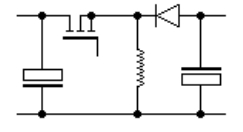
\includegraphics[width=4in]{includes/BuckBoost}
\caption{Buck-Boost Converter}
\end{center}
\end{figure}

\subsubsection{A flyback converter} 
``Several isolated output voltages, up to approximately 250 are possible''\cite{SMPSD}
\begin{figure}[H]
\begin{center}
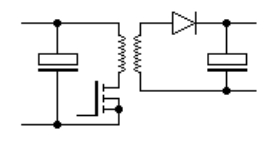
\includegraphics[width=4in]{includes/Flyback}
\caption{Flyback Converter}
\end{center}
\end{figure}

\subsubsection{Single Transistor Forward Converter} 
``One electrically isolated voltage, up to approximately 100 Watts.''\cite{SMPSD}
\begin{figure}[H]
\begin{center}
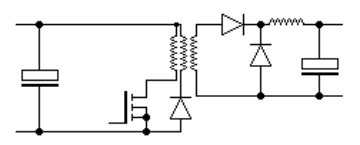
\includegraphics[width=4in]{includes/SingleTransistorFC}
\caption{Single Transistor Forward Converter}
\end{center}
\end{figure}


\subsubsection{Two Transistor Forward Converter}
 ``One electrically isolated voltage, up to approximately $1\kilo\watt$.''\cite{SMPSD}
\begin{figure}[H]
\begin{center}
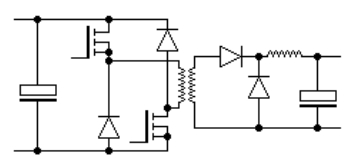
\includegraphics[width=4in]{includes/TwoTransistorFC}
\caption{Two-Transistor Forward Converter}
\end{center}
\end{figure}

\subsubsection{Half-Bridge Push-Pull Converter}
 ``One electrically isolated voltage, up to few kilo watts.''\cite{SMPSD}
\begin{figure}[H]
\begin{center}
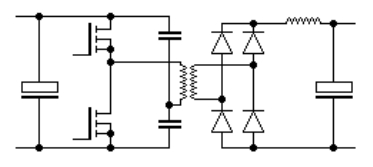
\includegraphics[width=4in]{includes/HalfBridgePushPullC}
\caption{Half-Bridge Push-Pull Converter}
\end{center}
\end{figure}

\subsubsection{Full-Bridge Push-Pull Converter}
 ``One electrically isolated voltage, up to many kilo watts.''\cite{SMPSD}
\begin{figure}[H]
\begin{center}
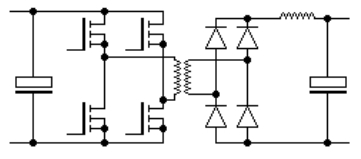
\includegraphics[width=4in]{includes/FullBridgePushPullC}
\caption{Full-Bridge Push-Pull Converter}
\end{center}
\end{figure}

%Source: \url{http://schmidt-walter.eit.h-da.de/smps\_e/smps\_e.html}

\subsection{Rating the Alternatives}
Once the team decided on a switched-mode supply, we needed to select a topology to use. The choices include a buck converter, a boost converter, a buck-boost converter, a flyback converter, single- and two-transistor forward converters, and half- and full-bridge push-pull converters. Some of these topologies can be eliminated immediately because the design will be too complex than needed to meet the needs of this design. For example, a boost converter takes the input voltage and converts it to a higher output voltage, which does not fit line voltage being converted to 5V DC. Similarly, a buck-boost converter outputs a negative voltage, which is also not fitting for this application. The single-transistor forward converter, two-transistor forward converter, half-bridge push-pull converter, and full-bridge push-pull converter have one electrically isolated voltage up to a varying number of watts. This would work for our design, however they are more complex than needed, other designs will work and be less complex. After these eliminations, the two remaining topologies are the flyback and the buck converters. The buck takes an input DC voltage and converts it into a lower output DC voltage, while a flyback can produce several isolated output voltages from an input AC voltage. Using a transformer and rectifier bridge can adapt an AC input into a DC voltage, allowing the buck topology to work where the flyback topology could also be used. Either design is feasible for the purpose specified. The flyback would use an inductor, while the buck uses a transformer. The team has used transformers for these purposes before, which would make the design easier. A flyback also can have multiple isolated voltages, but this was not needed in the design, so the team did not feel like this design was best. The team decided on a Buck Converter. Additionally,  Johnson Controls Incorporated graciously donated parts for a buck converter, as well as expert advice on designing and assembling one. As none of the members of the team have made a SMPS before, it felt very nice that the team could have an expert to go to for advice on a chip and design he has worked with several times.

\subsection{Implementation}
\subsubsection{Scope}
This section describes the analysis of the $5\volt/2\ampere$, LM25011-Buck Converter.
\subsubsection{Module Overview and Block Diagram}
\begin{figure}[H]
\begin{center}
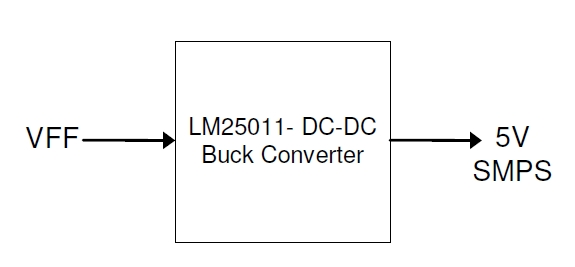
\includegraphics[width=4in]{includes/BlockDiagram}
\caption{Buck Conversion Use-Case Diagram}
\end{center}
\end{figure}

\clearpage
\subsubsection{Schematics}
\begin{figure}[htbp]
\begin{center}
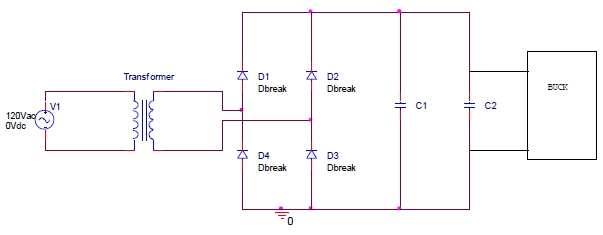
\includegraphics[width=6.5in,angle=90]{includes/ACtoDC}
\caption{Schematic of AC to DC Conversion}
\end{center}
\end{figure}

\begin{figure}[htbp]
\begin{center}
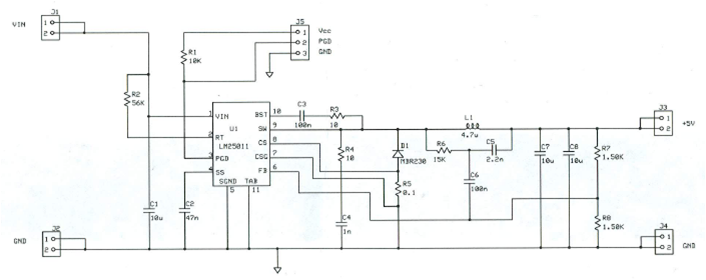
\includegraphics[width=6.5in,angle=90]{includes/Buck}
\caption{Schematic of Buck Converter DC to DC}
\end{center}
\end{figure}


\subsubsection{Calculations}
This power supply will require a transformer and four diodes as shown in the first schematic. These equations are for that part of the schematic.

\begin{equation}
V_{AC}=18 \volt
\end{equation}
 This is the voltage the transformer will output from a 120 $V_{AC}$ outlet. The buck converter needed at least 6V, but in order to be safe a transformer was chosen that was higher than this value. the buck converter could take up to 42V, so it was also safe from the maximum value.
\begin{equation}
Transformer_{peak}=VAC\sqrt{2}
\end{equation}
 Calculating for the rectifier circuit. This comes from the equation for finding $V_{rms}$, which is 
\begin{equation}
V_{rms}=\frac{V_p}{\sqrt{2}}
\end{equation}
$Current=2$ This is the desired output current. So, this is what I will equal in the following few equations.
\begin{equation}
dt=\frac{1}{120}\second
\end{equation} 
is the duration between charging cycles and is equal to 
\begin{equation}
\frac{1}{2\times Main \ \ Frequency}
\end{equation}
 Therefore since in America the main frequency is 60Hz, 
\begin{equation}
dt=\frac{1}{120}
\end{equation}
\begin{eqnarray}
Overhead&=&1.4\\
dv=Transformer_{peak}-Overhead-8&=&16.056
\end{eqnarray}

We need this $8\volt$ for the switching regulator, it needs $3\volt$ of headroom and since we want $5\volt$ out we take the voltage $+3\volt$ and get $8\volt$, but for a little bit of watermark/overhead.
\typeout{WHY DO WE HAVE A WATERMARK ON A VOLTAGE???? at \the\inputlineno\space in PowerSupply.tex}

\begin{equation}
Capacitor=Current\frac{dt}{dv}
\end{equation}
\begin{equation}
Capacitor=.001\farad
\end{equation}
 This simply means that the capacitor(s) for filtering need to be at least $1\milli\farad$.

\textbf{Note:This is a minimum value} This value could be achieved by one capacitor or multiple as long as the total capacitance is at least $1\milli\farad$.

The diodes were selected based on the fact that Chuck Howerda gave them to our team and said they would work well for this application and for the diode bridge.

%TODO: Fix Table, It is too big for page.
\subsubsection{Capability Justification Table}
{
\begin{longtable}[c]{|p{1.5in}|c|c|c|}
%% Longtable setup
\caption{Power Supply Capabilities} \\ \hline
Capability Parameter & Specification & Analysis Result & Remarks \\ \hline
\endfirsthead
\caption[]{Continued from previous page} \\ \hline
Capability Parameter & Specification & Analysis Result & Remarks \\ \hline
\endhead

\multicolumn{4}{r}{{Continued on next page}} \\
\endfoot

\endlastfoot

%% Longtable content
Input Voltage & Min & $7.09\volt$ & From Current Draw \\ \hline
Input Voltage & Max & 17.10\volt & From Current Draw \\ \hline
Switching Frequency & Max & 3.38\mega\hertz & From Current Draw \\ \hline
Output Voltage & Min & 4.99\volt & From Calculation \\ \hline
Output Voltage & Max & 5.19\volt & From Calculation \\ \hline
Output Ripple Voltage & Max & 10\milli\volt & Assumed \\ \hline
Output Current & Max & 2\ampere & From Current Draw \\ \hline
Output Inductor & Typ & 2.2\micro\henry & From Schematic \\ \hline
Power Dissipation across Inductor & Max & 99\milli\watt & From Calculation \\ \hline
Power Dissipation across current sense resistor during current limit mode & Max & 246\milli\watt & From Calculation \\ \hline
Efficiency & Max & 86.86\percent & From Calculation \\ \hline
Softstart Time & Min & 8.032\milli\second & From Calculation \\ \hline
Softstart Time & Max & 12.048\milli\second & From Calculation \\ \hline
Input Under Voltage Protection Threshold & Min & 4.6\volt & From Datasheet \\ \hline
Thermal Shutdown & Typ & 155\degree C & From Datasheet \\ \hline
Line Regulation & Max & 5 +/- 5\percent & Verify by Testing \\ \hline
Load Regulation & Max & 5 +/- 5\percent & Verify by Testing \\ \hline
Gain Margin &  &  & Verify by Testing \\ \hline
Phase Margin &  &  & Verify by Testing \\ \hline
%\end{tabular}
%\end{center}
%\label{default}
%\end{table}%
\end{longtable}
} 
This table was co-produced with Hilbrand Sybesma, a hardware engineer at JCI. After we were both done working on January 27, 2011, he took the time to work with me on them. As I was creating it, he stopped me if I made any errors and he told me other things to include. He went above and beyond with help. 

\subsubsection{Theory of Operation}
"The LM25011 Constant On-time Step-Down switching regulator is capable of supplying up to $2\ampere$ of load current. This high voltage regulator contains an N-Channel Buck switch, a startup regulator, current limit detection,and internal ripple control. The constant on-time regulation principle requires no loop compensation, results in fast load transient response, and simplifies circuit implementation.


The operating frequency remains relatively constant with line and load. The adjustable valley current limit detection results in a smooth transition from constant voltage to constant current mode, when current limit is reached, without the use of current limit foldback. The PGD output indicates the output voltage has increased to within $5\percent$ of the expected regulation value.

Additional features include: Low output ripple, VIN under-voltage lock-out, adjustable soft-start timing, thermal shutdown, gate drive pre-charge, gate drive under-voltage lock-out, and maximum duty cycle limit."\cite{LM25011}
%Source: \url{http://www.national.com/pf/LM/LM25011.html\#Overview}
\subsubsection{Design Assumptions}
 VFF value is considered as min. $7.09\volt$ and max. $17.10\volt$ from Current draw of the chip in use.
\subsubsection{Analysis}
\begin{outline}[enumerate]
\1 Input voltage range:
\begin{equation}
P_{VFF}=7.09, 12.3, 17.1 \volt
\end{equation}
\2 Input Voltage range for the LM25011 is $6\volt$ to $42\volt$ 12.3V was choosen for a medium between 7.09 and 17.1.
\1 Output Voltage
\begin{equation}
P_{5V}=4.75, 5, 5.25 \volt
\end{equation}
\2 These values are from the 5\percent tolerance. 
\1 Load Current
\begin{equation}
I_{out}=2\ampere
\end{equation}
\2 Note: As per datasheet, LM25011 can deliver up to 2\ampere load current \cite{LM25011}.
\end{outline}


\subsubsection{Output Voltage Calculation}
Calculations from datasheet:
\begin{figure}[htbp]
\begin{center}
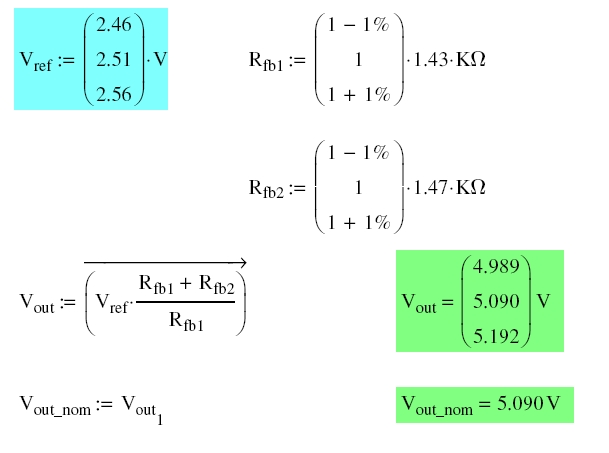
\includegraphics[width=3in]{includes/DatasheetCalc}
\caption{Calculation from datasheet}
\end{center}
\end{figure}


\subsubsection{Selection of Switching Frequency}
Information from datasheet:

The maximum allowed frequency may be limited by the minimum and maximum input voltage, as described below:
\begin{outline}[enumerate]
\1 Operation at a low input voltage requires a high duty cycle to maintain output regulation. The maximum duty cycle is limited by the minimum off-time of the LM25011 (150ns typ., 208 ns max).  The output voltage drops out of regulation at low VIN if  the switching frequency does not satisfy the following condition:
\begin{equation}
Fsw < (Vin(min)-Vout) / ( Vin(min) x 208ns)
\end{equation}
\1 Operation at high input voltage requires a low duty cycle, limited by the minimum on-time of the LM25011 (90 ns). The switching frequency must satisfy the following condition to ensure the on-time is greater than 90 ns:
\begin{equation}
Fsw < Vout / (Vin(max) x 90ns)
\end{equation}
\end{outline}

If the selected value of Fsw does not satisfy this condition, the LM25011 maintains regulation, but the switching frequency will be lower than the desired value.

\begin{figure}[htbp]
\begin{center}
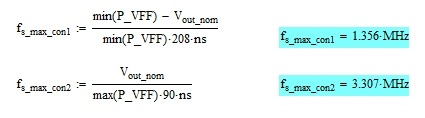
\includegraphics[width=6in]{includes/freq}
\caption{Condition from datasheet}
\end{center}
\end{figure}

From the conditions shown, maximum switching frequency should not exceed $1.356 \mega\hertz$.

The approximate operating frequency is calculated as follows:
\begin{equation}
RT_{used}=\left( \begin{array}{ccc}
1-1\percent \\ 1 \\ 1+1\percent \\
\end{array} \right)
\end{equation}
\begin{equation}
V_in=P_{VFF}
\end{equation}

\begin{equation}
f_s=\frac{V_{out->nominal}}{(V_{in}15ns)+[4.1*10^{-11}(RT_{used}+.5\kilo\ohm)\ampere\second]}
\end{equation}
\begin{equation}
f_s=\left( \begin{array}{ccc}
2.121 \\ 2.035 \\ 1.961 \\ 
\end{array} \right)
\end{equation}
\begin{equation}
f_{sMAX}=2\mega\hertz \quad \hbox{From Datasheet}
\end{equation}

For the selected RT value, switching frequency is higher than 2MHz. However after speaking with the contact from National Semiconductor I have confirmed that LM25011 can operate up to 2.4MHz.

\subsubsection{Selection of Inductor}
As per JCI recommendations as well as National Semiconductor, we opted to use a 15\micro\henry inductor since they said it is the best to use because we will want more than the minimum requirement. 

\subsubsection{Ripple Current}
\begin{outline}[enumerate]
\1 Maximum Ripple Current
\begin{equation}
I_{ripple\_max}=(max(V_{in})-min(V_{out}))(\frac{min(T_{on\_min})}{min(L{recom})})
\end{equation}
\2 Note: This is acceptable.
\begin{equation}
I_{ripple\_max}=294.851\milli\ampere
\end{equation}
\1 Nominal Ripple Current
\begin{eqnarray}
I_{ripple\_nom}&=&(V_{in_1}-V_{out})(\frac{min(T_{on\_min})}{min(L{recom})})\\
I_{ripple\_nom}&=&175.525\milli\ampere
\end{eqnarray}
\1 Minimum Ripple Current
\begin{eqnarray}
I_{ripple\_min}&=&(min(V_{in})-max(V_{out}))(\frac{min(T_{on\_min})}{min(L{recom})})\\
I_{ripple\_min}&=&95.321\milli\ampere
\end{eqnarray}
\1 Inductor Peak Current
\begin{eqnarray}
I_{peak}&=&I_{out\_max}+\frac{I_{ripple\_max}}{2}\\
I_{peak}&=&2.147\ampere
\end{eqnarray}
\end{outline}

\subsubsection{Minimum Valley Threshold for Current Limit}
\begin{equation}
I_{valley\_th}=I_{out\_max}-\frac{I_{ripple\_min}}{2}
\end{equation}

\subsubsection{Current Sense Resistor}
As long as we have a current sense resistor that does not exceed $RS_{max}$ (located in the datasheet) it will be okay. The more current we want in our power supply the smaller our current sense resistor will need to be. Which we can vary as we see fit. The proportion to which this varies depends on the ripple voltage and the calculation for which is shown below.


\subsubsection{Ripple Voltage}
\begin{eqnarray}
RS_{ripple\_min}&=&min(RS_{used})min(I_{ripple\_min})\\
RS_{ripple\_min}&=&10.381 \milli\volt
\end{eqnarray}
As per datasheet, minimum ripple voltage across current sense resistor should be greater than $10\milli\volt$. In this case it is very close, but that should not be a problem.

\subsubsection{Power Dissipation}
We set the current sense resistor to get 1.5A out. Also, by the results of the testing we get 1.3A out instead of 1.5A. We still get 5V out. Therefore we can calculate the efficiency.
\begin{eqnarray}
Eff&=&\frac{P_{out}}{P_{in}}\\
Eff&=&\frac{1.3 \times 5}{1.5 \times 5}\\
Eff&=&88.7\% +/- 5\%
\end{eqnarray}

So, therefore $Eff=84.23\percent,\ \ 88.7\percent,\ \ 93.1\percent$

\subsubsection{Efficiency}
No adequate information is provided in the datasheet about power loss in LM25011, However to identify approximate power loss in LM25011, the Efficiency of the LM25011 buck converter is simulated using National Semiconductor Webench tool for the same specification.\cite{WEBENCH}

\begin{figure}[htbp]
\begin{center}
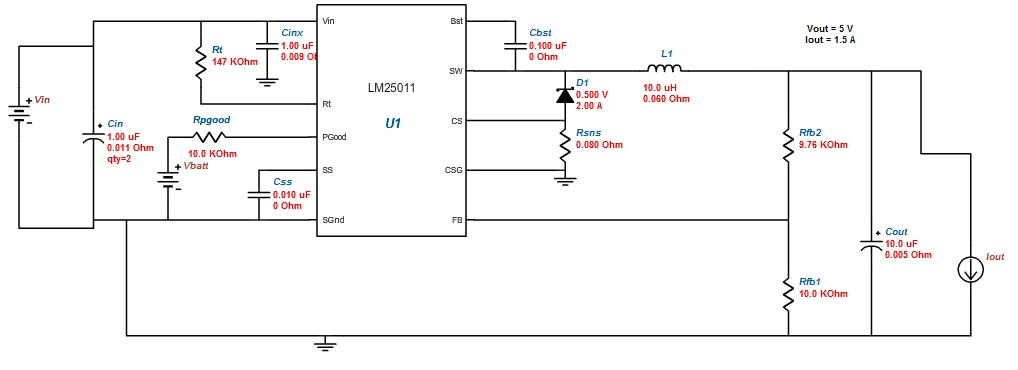
\includegraphics[width=5in]{includes/WebenchCircuit}
\caption{Circuit as shown in Webench}
\end{center}
\end{figure}

\begin{figure}[htbp]
\begin{center}
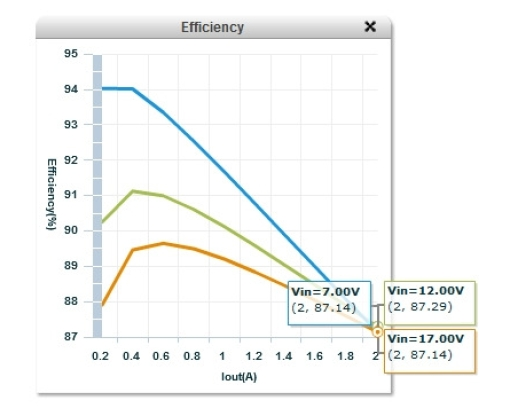
\includegraphics[width=4in]{includes/eff}
\caption{LM25011 Efficiency graph from Webench tool $Eff=86.85\percent$}
\end{center}
\end{figure}


\subsubsection{Total Output Power}
\begin{eqnarray}
P_{out}&=&max(V_{out})I_{out\_max}\\
P_{out}&=&10.383\watt\\
P_{in}&=&\frac{P_{out}}{Eff}\\
P_{in}&=&11.955\watt
\end{eqnarray}

\subsubsection{Approximate power loss in LM25011}
\begin{eqnarray}
PD_{LM25011}&=&P_{in}-PD_{ext}-P_{out}\\
PD_{LM25011}&=&223.948\milli\watt
\end{eqnarray}

\subsection{Testing}
First I tested just the power supply with no load to make sure it gave a $5\volt$ output, which was measured with a DMM. That was a success! After which, I put a load of $2.5\ohm$ to see how much current went through. Those values and test setup are shown in the pictures as follows:
% Section only contains relevent pictures...more are in the appendix
\begin{figure}[htbp]
\begin{center}
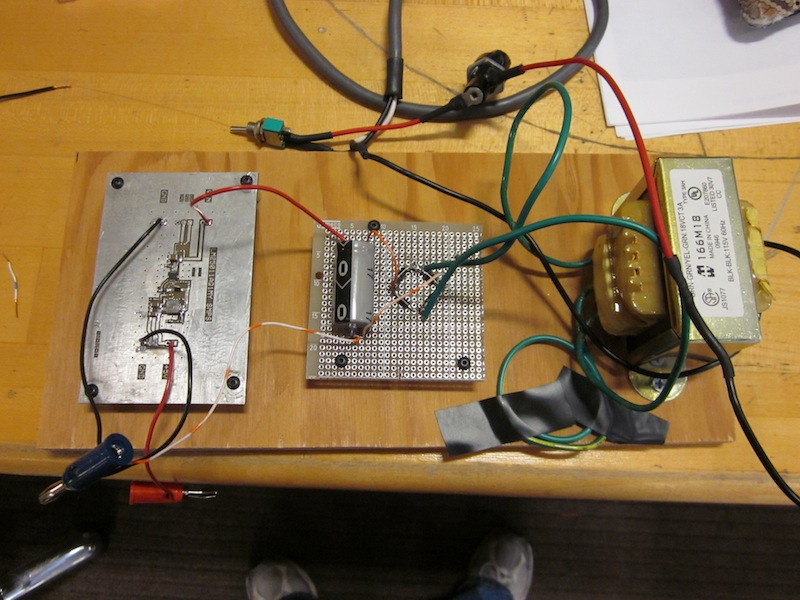
\includegraphics[width=4in]{includes/IMG_0262}
\caption{Full Assembly}
\end{center}
\end{figure}

\begin{figure}[htbp]
\begin{center}
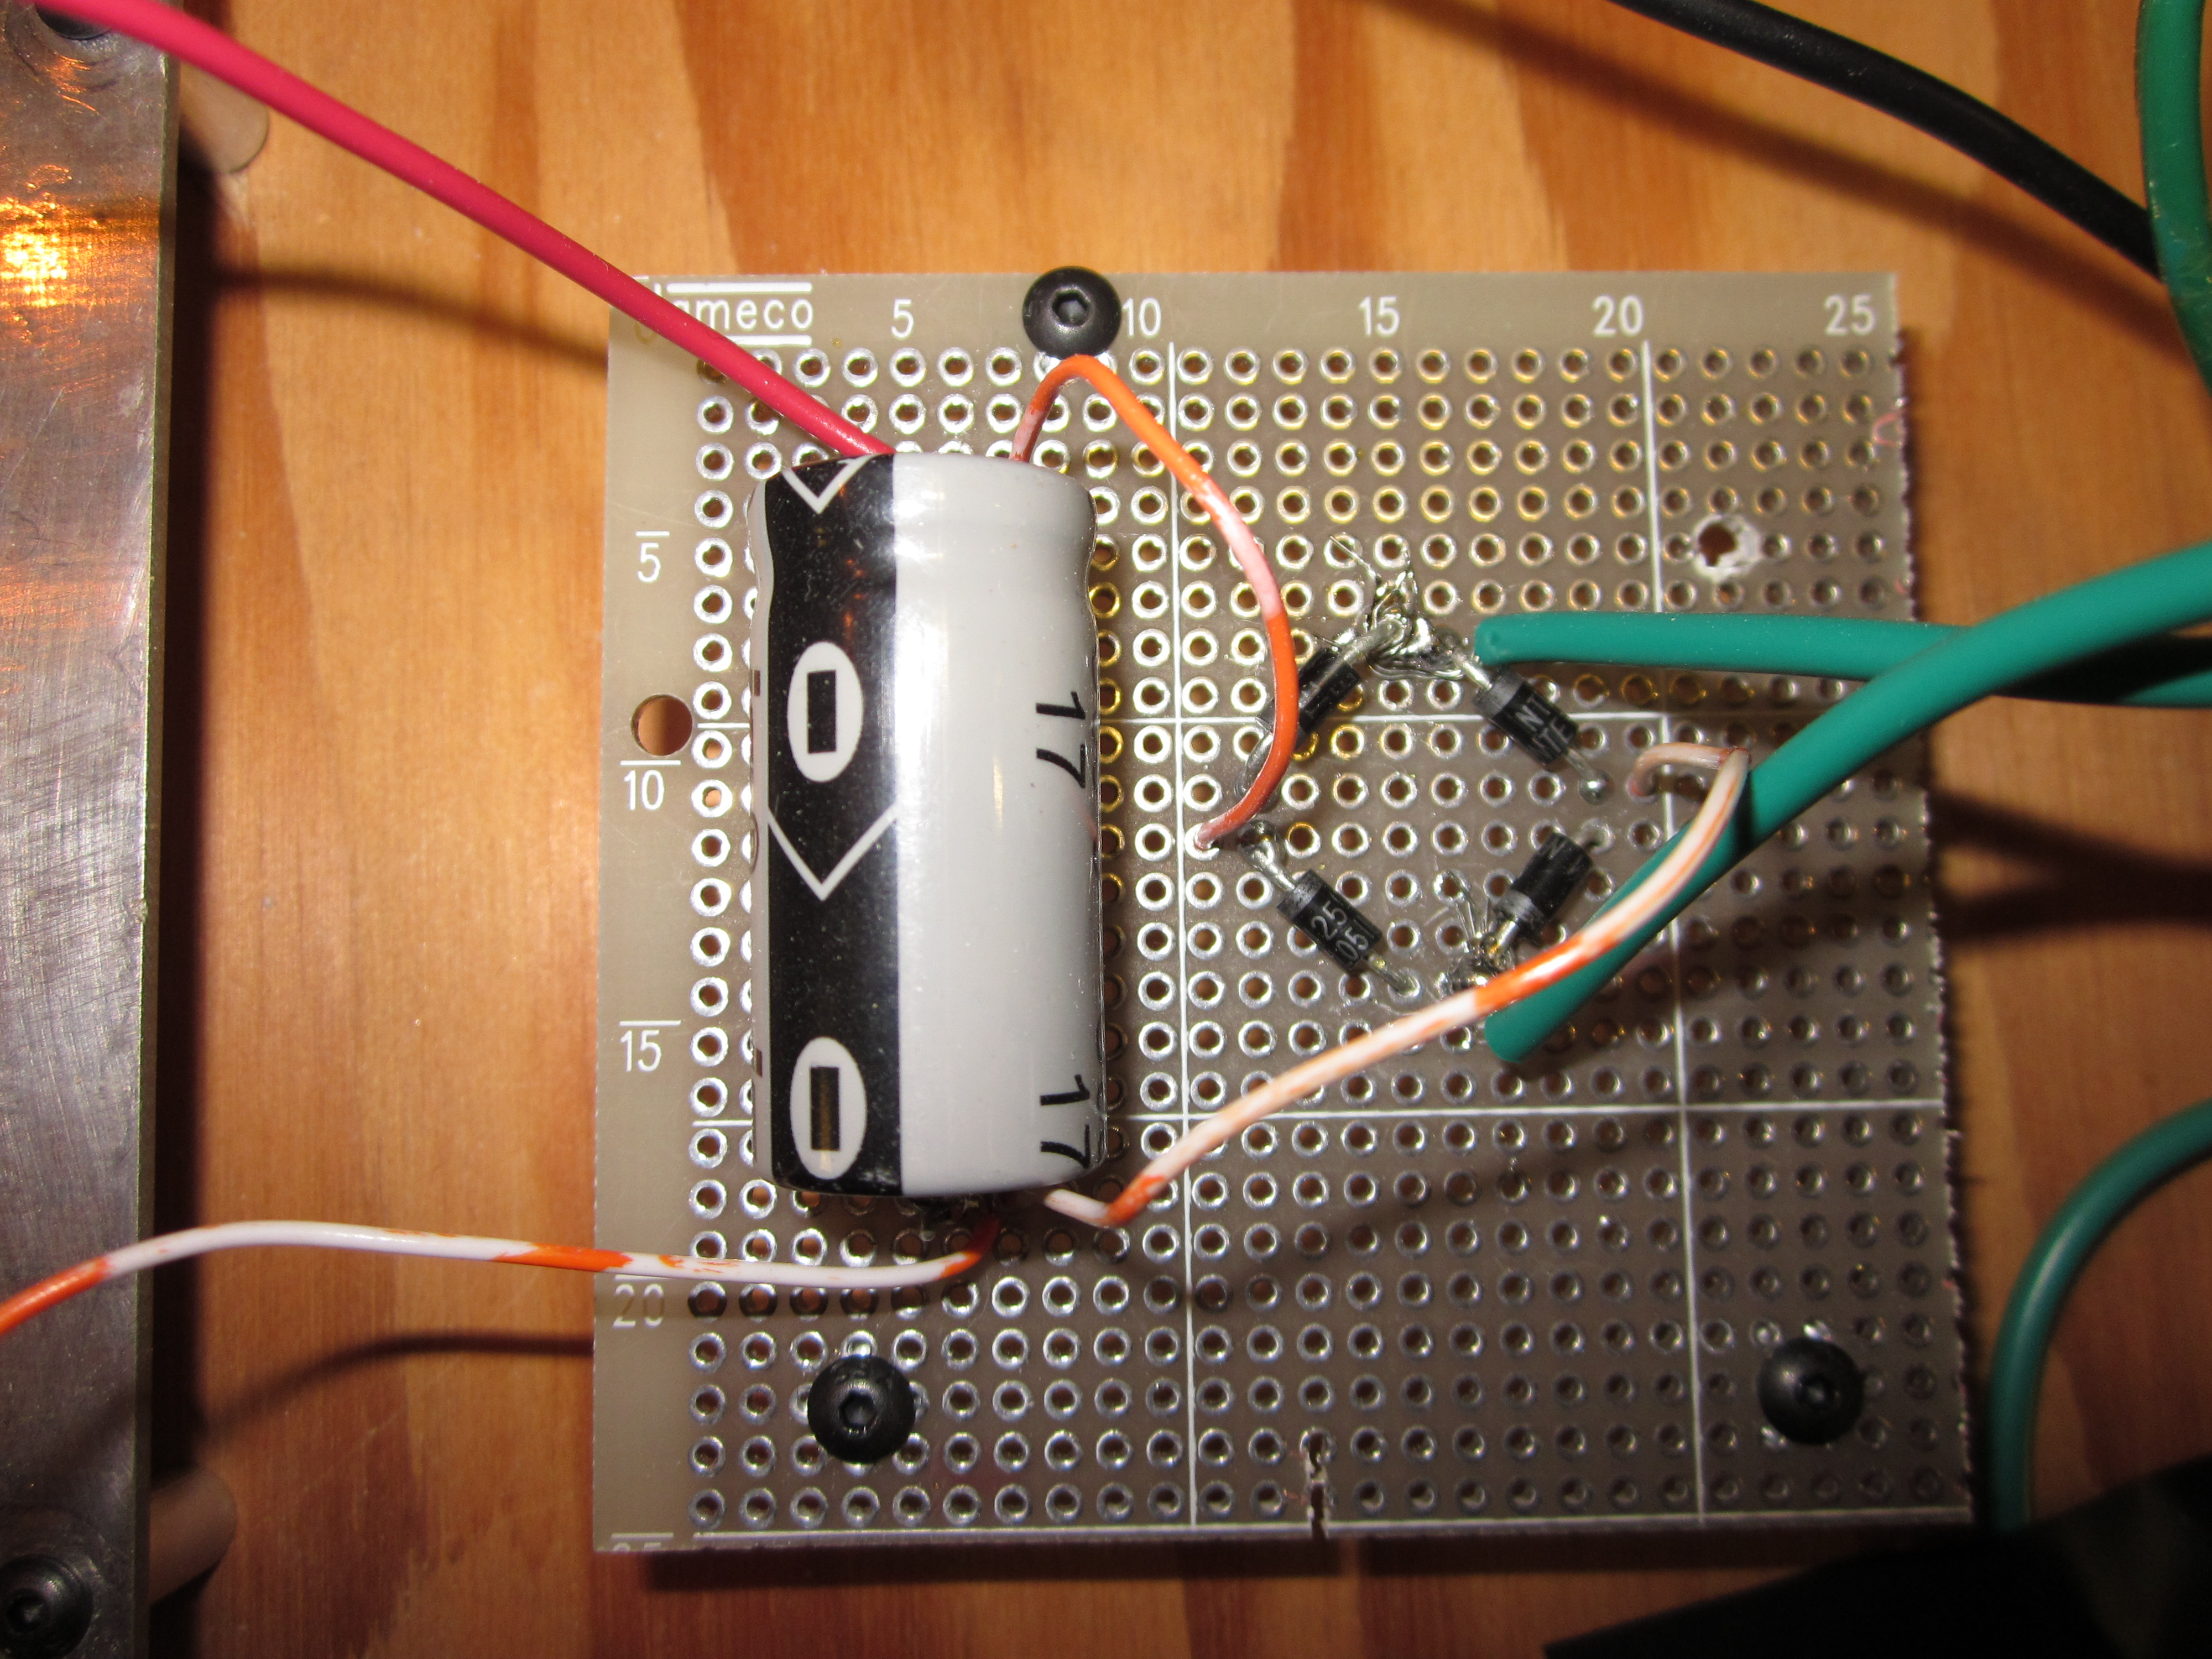
\includegraphics[width=4in]{includes/IMG_0264}
\caption{Rectifier Circuit}
\end{center}
\end{figure}

\begin{figure}[htbp]
\begin{center}
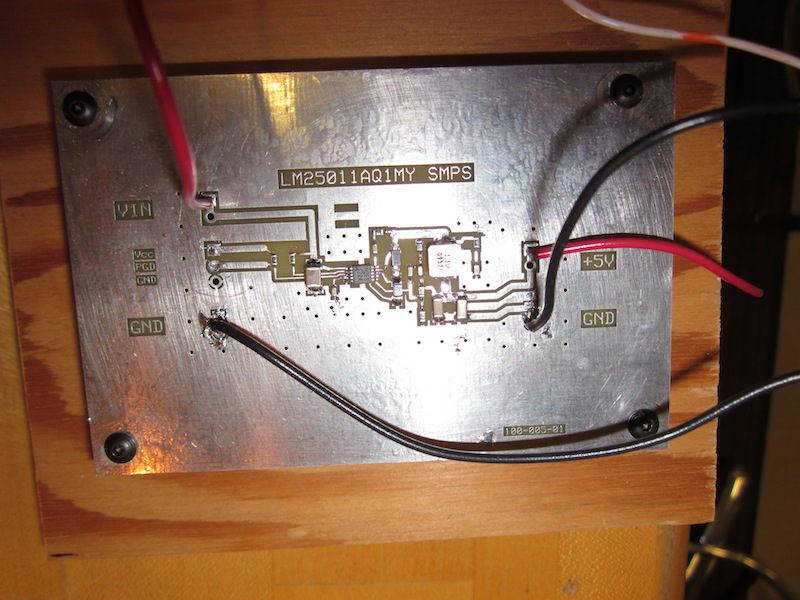
\includegraphics[width=4in]{includes/IMG_0263}
\caption{Buck Converter}
\end{center}
\end{figure}


%%%%%%%%%%%%%%%%%%%%%%%%%%%%%%%%%%%%%%%%%%%%%%%%%%%%%%%%%%%%%
